\section{Application: Finding Completions of Underconstrained Glassy Structures from Underconstrained to Isostatic}
\label{sec:bodypin}

% \bibliography{paper}



\ClearMyMinHeight
\SetMyMinHeight{.3}{../../img/silica}
\SetMyMinHeight{.2}{../../img/Silicon_tetrahedron}

\begin{figure}\centering
    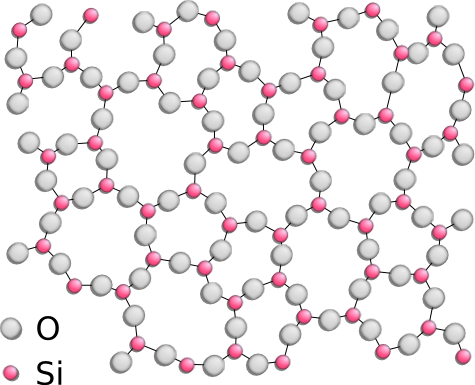
\includegraphics[height=\myMinHeight]{../../img/Silica}
    \hspace{0.5cm}
    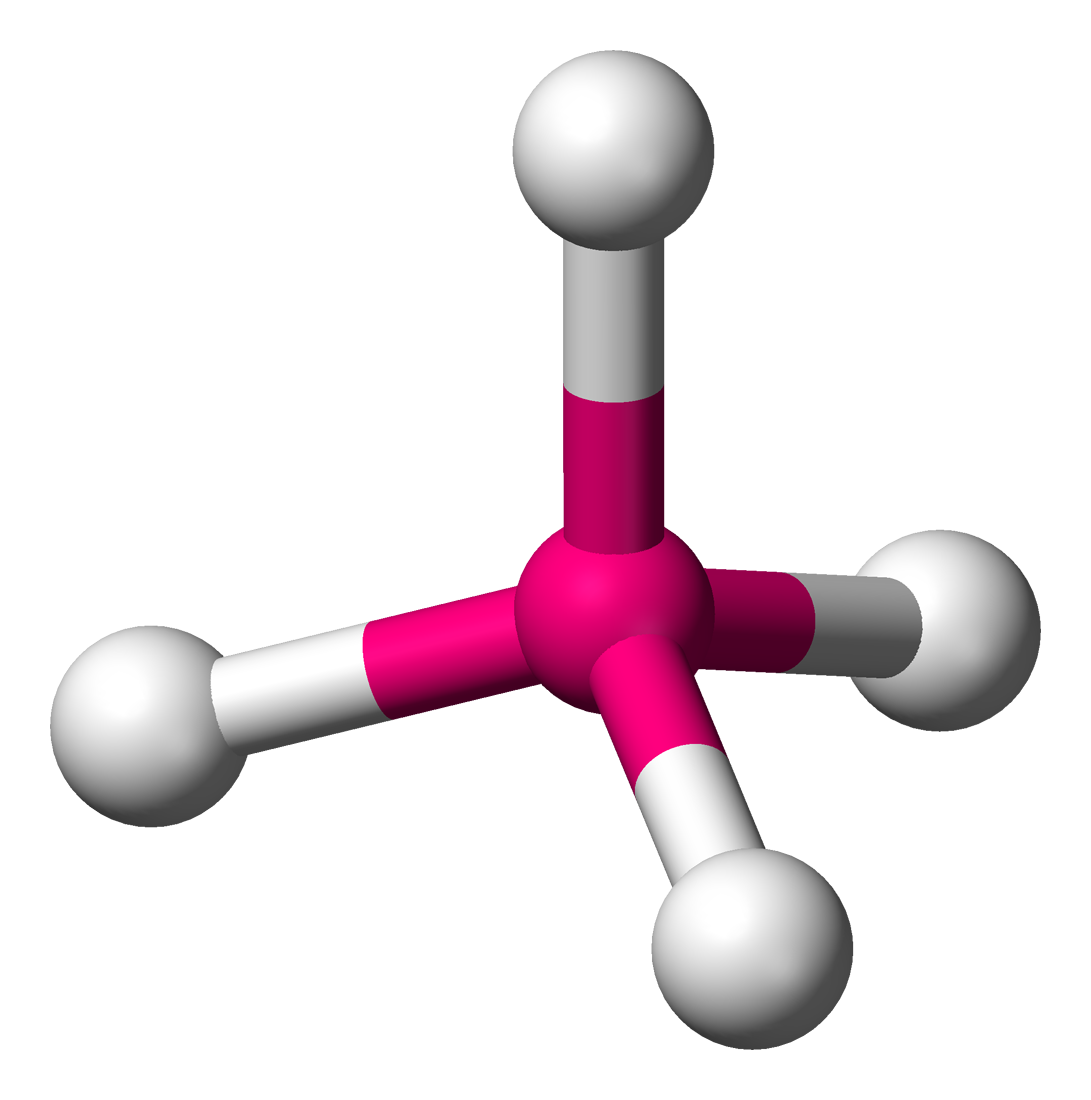
\includegraphics[height=\myMinHeight]{../../img/Silicon_tetrahedron}
    % \raisebox{0.25\height}{
    %     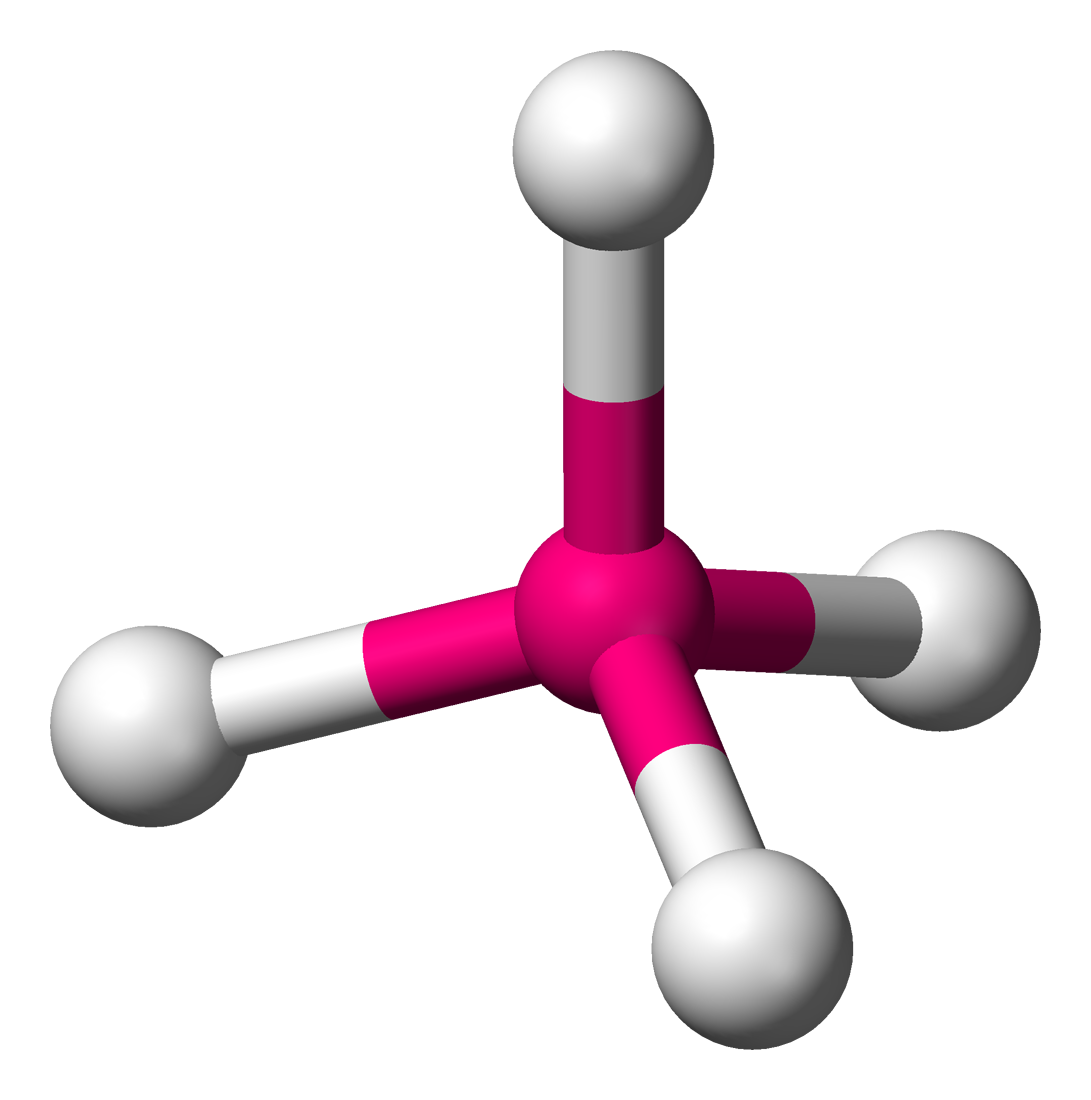
\includegraphics[height=\myMinHeight]{../../img/Silicon_tetrahedron}
    % }
    \caption{Example of a single monolayer of a silica (silicon and oxygen) glassy structure. This can be viewed as a triangle-multipin qusecs where the silicon atoms are the triangles and the oxygen atoms are the pins. Not shown here are other monolayers stacked on this one. Each silicon atom has the structure seen to the right, and so binds to another oxygen atom in an adjacent monolayer. Pictures taken from \cite{silica_figure} and \cite{tetra_silica_figure}.}
    \label{fig:silica_glass}
\end{figure}


We can use qusecs DR-plans to design materials such as disordered graphene and silica bi-layers \cite{silica_bilayers} \cite{sructure_of_2d_glass}. We investigate a more specific problem in a somewhat more general setting: the problem of finding boundary conditions (additional constraints) to add to an underconstrained monolayer to make it isostatic. This can be done in a number of ways: (1) pin together 2 underconstrained monolayers in such a way that the resulting bi-layer becomes isostatic (see Figure \ref{fig:silica_glass}); (2) pin the boundary of (or in general, add constraints to) a layer (possibly a genus 0 monolayer) so that it becomes isostatic; or (3) design a broader class of structures to ensure they are isostatic, self-similar (via some subdivision rule) and in addition isostatic at each level of the subdivision (see Figure \ref{fig:subdivision}).

In all cases, we are specifically interested in how to add additional constraints such that the resulting isostatic structure has a small DR-plan; this way a realization can be found, allowing efficient stress, flex and other property design related to the rigidity matrix. To answer these questions, we first introduce the qusecs that are used to model these materials. In this section, we discuss Item (2) in detail.

% \begin{figure}\centering
%     (a)
%     \begin{subfigure}{0.2\linewidth}
%         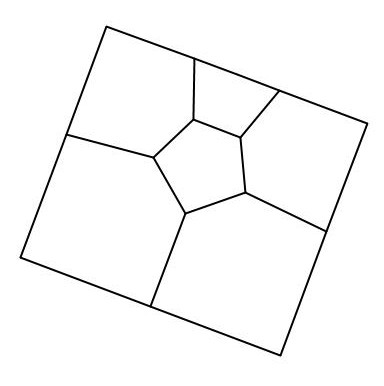
\includegraphics[width=\linewidth]{../../img/pentl1}
%     \end{subfigure}
%     %
%     $\rightarrow$
%     \begin{subfigure}{0.2\linewidth}
%         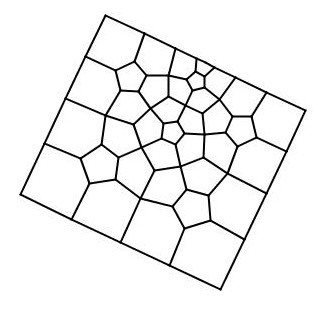
\includegraphics[width=\linewidth]{../../img/pentl2}
%     \end{subfigure}
%     %

%     (b)
%     \begin{subfigure}{0.8\linewidth}
%         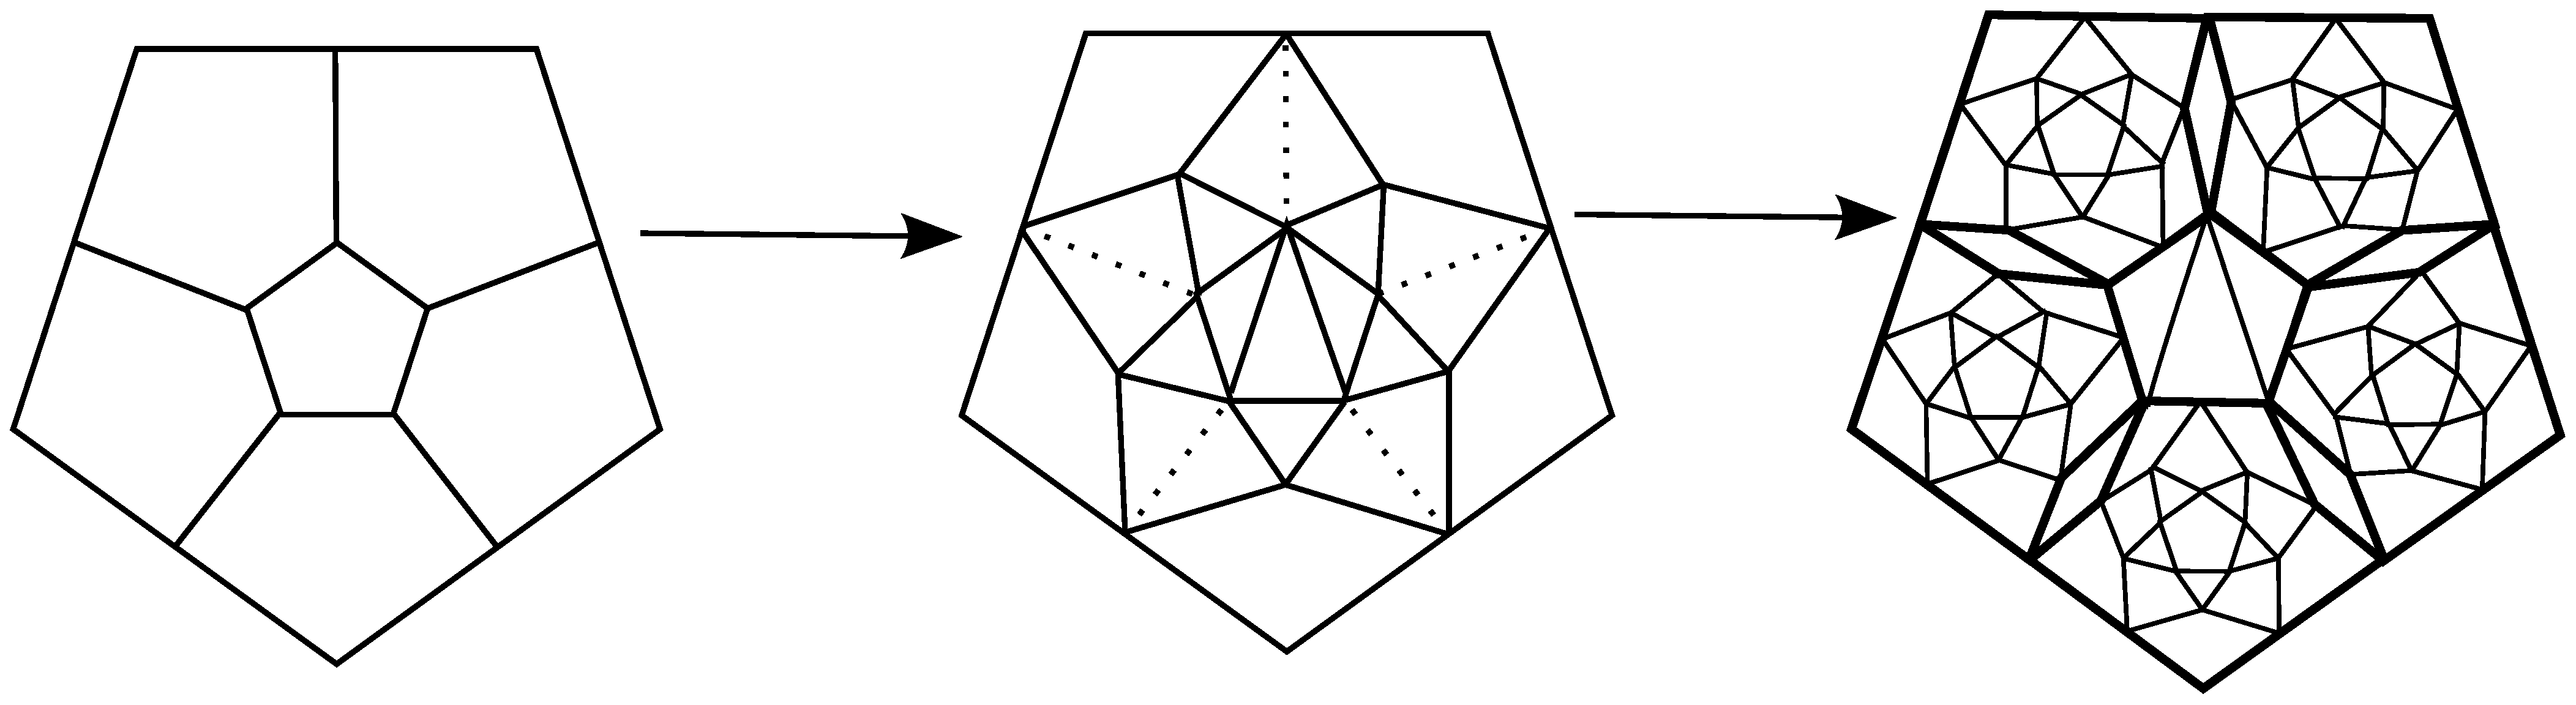
\includegraphics[width=\linewidth]{../../img/pentawesome}
%     \end{subfigure}
%     \caption{Examples of self-similarity via repeated subdivision. In (a), simple subdivision that does not guarantee isostaticity. In (b), a more complicated scheme is used, ensuring that the resulting graph is isostatic but not  tree-decomposable. Credit to \cite{subdivision_paper} for (a).}
%     \label{fig:subdivision}
% \end{figure}


\begin{figure}\centering
    \begin{subfigure}{0.35\linewidth}
        $
        \vcenter{\hbox{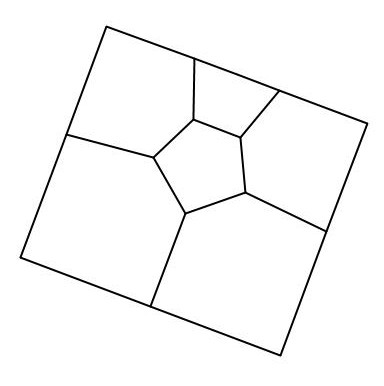
\includegraphics[width=.4\linewidth]{../../img/pentl1}}}
        % \raisebox{-.5\height}{\scalebox{1}{$\rightarrow$}}
        \vcenter{\hbox{$\rightarrow$}}
        \vcenter{\hbox{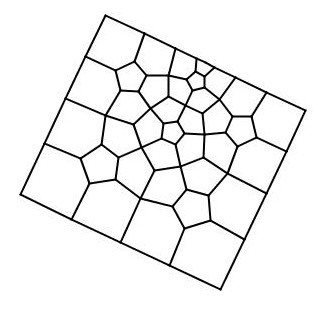
\includegraphics[width=.4\linewidth]{../../img/pentl2}}}
        $
        \caption{}\label{fig:subdivision:simple}
    \end{subfigure}
    \begin{subfigure}{0.55\linewidth}
        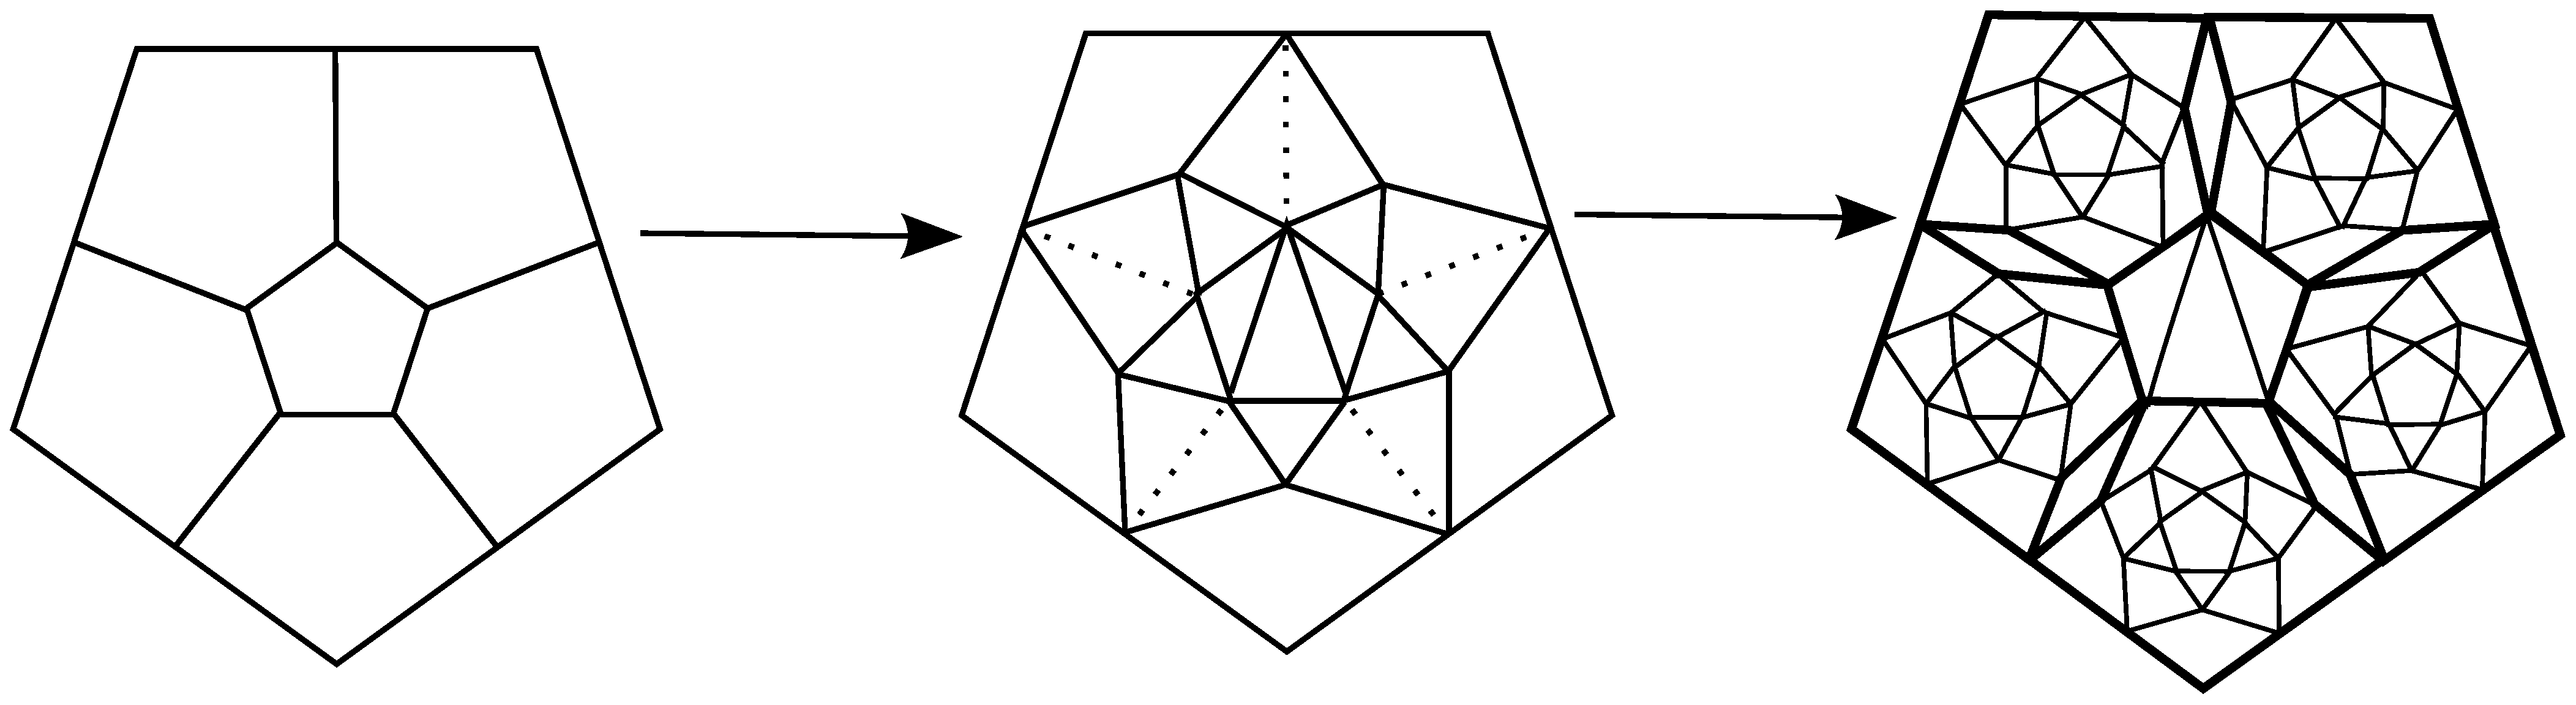
\includegraphics[width=\linewidth]{../../img/pentawesome}
        \caption{}\label{fig:subdivision:complicated}
    \end{subfigure}
    \caption{Examples of self-similarity via repeated subdivision. In (\ref{fig:subdivision:simple}) \cite{subdivision_paper}, there is a simple subdivision scheme that does not guarantee isostaticity. In (\ref{fig:subdivision:complicated}), a more complicated scheme is used, ensuring that the resulting graph is isostatic but not  tree-decomposable.}
    \label{fig:subdivision}
\end{figure}

\subsection{Body-Hyperpin Qusecs}


% \begin{definition}
%     A \dfn{body-hyperpin qusecs} is a constraint system where the objects are rigid bodies, subsets of which are pinned together by pins (i.e.\ they are incident at a common point.)
% \end{definition}

\begin{definition}
[Body-hyperpin qusecs]
    A \dfn{body-hyperpin qusecs} is a constraint system where the objects are rigid bodies and the constraints are incidences of object subsets at a common point, i.e.\ a pinning of bodies.
\end{definition}

\begin{remark*}
\label{rem:bodypin_is_barjoint}
    A body-hyperpin qusecs is a special case of bar-joint qusecs of the previous sections of the paper. As such, the DR-planning for isostatic systems discussed in Section \ref{sec:DRP} is unchanged and the results of Section \ref{sec:recomb} still go through with minor modifications.
\end{remark*}

For the remainder of this section, we deal only with the DR-plan of such qusecs. Hence, we refer only to the combinatorics or underlying hypergraph of the qusecs. We now introduce 2 sub-classes of body-hyperpin graphs for modeling Examples 4 and 5 in Section \ref{sec:intro}, for which the optimal completion problem is significantly easier.

\begin{definition}
[Body-pin graph]
\label{def:body-pin}
    A \dfn{body-pin graph} is a body-hyperpin graph with the following conditions:
    (1) each pin is shared by at most two bodies; and
    (2) no two bodies share more than one pin

    Such a body-pin graph, $G_{BP}$, can also be seen as a \dfn{body-bar graph}, $G_{BB}$, where the bodies of $G_{BB}$ are the original bodies of $G_{BP}$ and each pin between bodies in $G_{BP}$ are replaced with 2 bars in $G_{BB}$ between the same bodies.
    Such body-bar graphs with 1 and 2-dof can be characterized by being $(3,4)$ and $(3,5)$-tight respectively \cite{Lee:2007:PGA} \cite{streinu2009sparse} (defined in \ref{sec:appendix:defs}). See Figure \ref{fig:bodypindrp:b}.
\end{definition}

\begin{definition}
[Triangle-hyperpin graph]
    A \dfn{triangle-hyperpin graph} is a body-hyperpin graph where each body is a triangle, i.e.\ it shares  pins with at most 3 other bodies. This is also represented as a hyper-graph where each pin is a vertex and each triangle represents a tri-hyperedge. For such hypergraphs, {\em 1 and 2-dof} can be characterized by $(2,4)$ and $(2,5)$-tightness respectively \cite{Lee:2007:PGA} \cite{streinu2009sparse}.
\end{definition}

Body-pin graphs are of particular interest to us in the context of Example 4 in Section \ref{sec:intro}. Triangle-multipin graphs can be used to represent the silica bi-layers and glassy structures described in Example 5 of Section \ref{sec:intro}, where each triangle is the junction of ``disks'' in the plane (see Figure \ref{fig:silica_glass}). Typically, these systems are not isostatic, so to relate the work of this paper to the systems, we define a slightly different kind of DR-plan using the notion of $(k,l)$-sparsity and tightness.

\begin{definition}
[$(k,l)$-tight DR-plan]
    A \dfn{$(k,l)$-tight DR-plan} is one in which each child node is either a vertex maximal proper $(k,l)$-tight subgraph of the parent node or it is trivial. In our case, the trivial nodes are the bodies.
\end{definition}

Provided such $(k,l)$-sparse graphs are matroidal (conditions given in \cite{Lee:2007:PGA}),
the notion of a canonical DR-plan extends directly to the case when the hypergraph is $(k,l)$-sparse (i.e.\ independent) using the straightforward notion of trivial and non-trivial intersections and $(k,l)$-tightness conditions as in Section \ref{sec:DRP}. In particular, we define canonical DR-plans with similar properties for the 1 and 2-dof body-pin and triangle-hyperpin systems defined above.

\begin{observation*}
\label{obs:bodypin_drp}
    For the 1-dof body-pin graphs described above that are $(3,4)$-sparse, a $(3,4)$-tight canonical DR-plan exists where every node of a $(3,4)$-sparse graph satisfies one of the following: (1) its children are 2 proper vertex-maximal 1-dof graphs that intersect on another 1-dof graph; or (2) its children are all of the proper maximal 1-dof subgraphs, pairwise sharing at most one body.
\end{observation*}

% \begin{observation}
% \label{obs:bodypin_drp}
%     For the 1-dof body-pin graphs described above, $(3,4)$-sparsity corresponds to a canonical DR-plan whose nodes satisfy one of the following, either
%     (a) the children are 2 proper vertex maximal 1-dof graphs that intersect on another 1-dof graph, or
%     (b) the children are a number of proper maximal 1-dof subgraphs, sharing at most one body.
% \end{observation}

% \begin{proof}
%     \todo{Item 1 Follows from paper?}

%     For item 2, consider the case where we have more than 2 proper vertex maximal 1-dof subgraphs $s_1, ..., s_k, k > 2$. Then, if $k_i$ and $k_j$ are joined by $2$ pins, $k_i \cup k_j$ would be $(3,4)$-tight and hence $k_i$ and $k_j$ are not vertex maximal.
% \end{proof}

As in Section \ref{sec:DRP},  a strong Church-Rosser property holds, making all canonical DR-plans optimal:
%
\begin{observation*}
\label{rem:1dofcanon}
    When the input is independent, all $(3,4)$-tight canonical DR-plans are optimal. We can find such a DR-plan in the same time complexity as the $(2,3)$-tight case for bar-joint graphs discussed in Section \ref{sec:DRP}.
\end{observation*}

The above-mentioned algorithm exists because such $(3,4)$-tight graphs are matroidal and have a pebble game \cite{Lee:2007:PGA}.

\ClearMyMinHeight
\SetMyMinHeight{.2}{../../img/bodypin}
\SetMyMinHeight{.2}{../../img/epsfromtikz/bodypin_graph}
\SetMyMinHeight{.35}{../../img/epsfromtikz/bodypin_drp}
\SetMyMinHeight{.2}{../../img/bodypin2}

\begin{figure*}\centering
    \begin{subfigure}{0.2\linewidth}\centering
        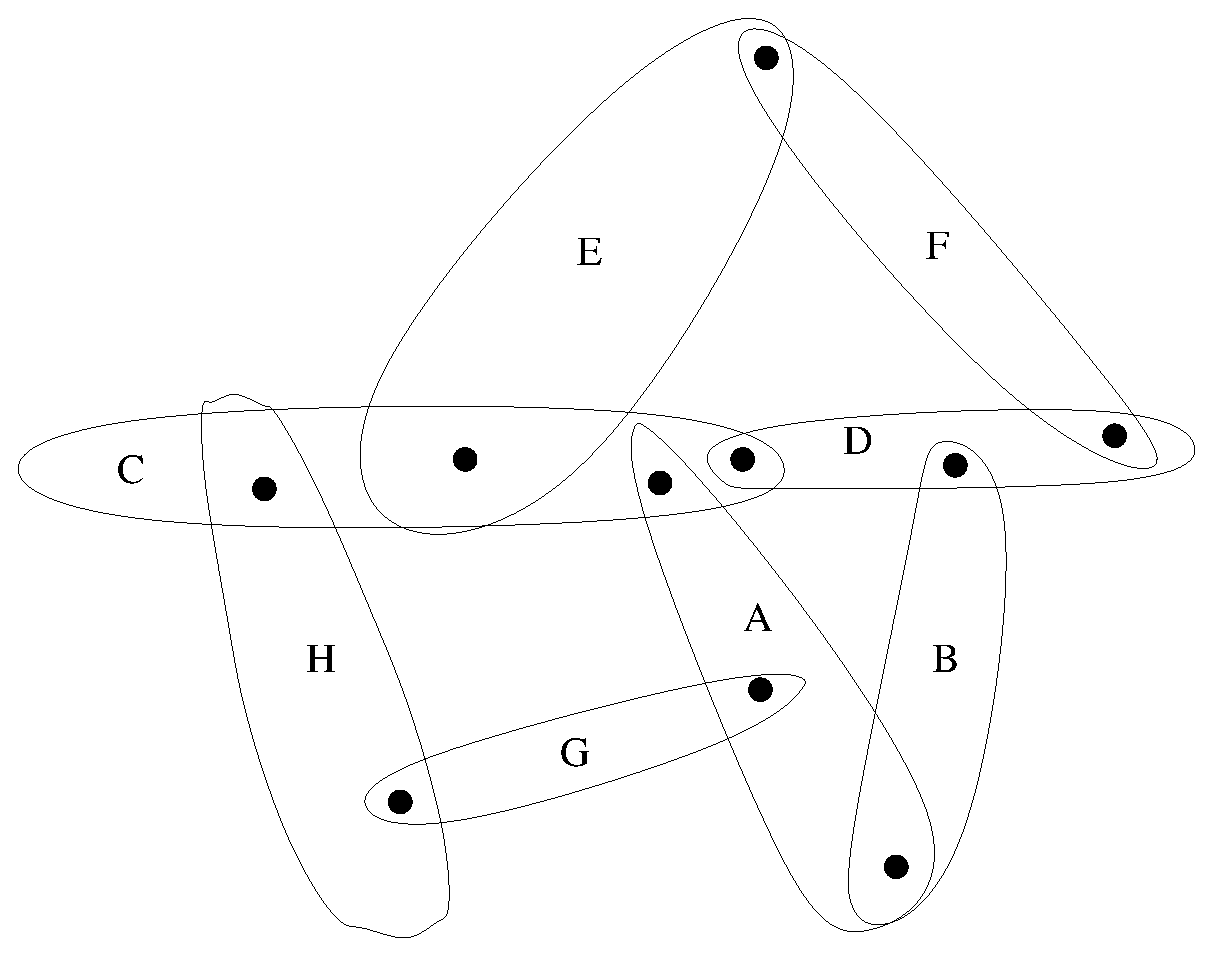
\includegraphics[height=\myMinHeight]{../../img/bodypin}
        \caption{}\label{fig:bodypindrp:a}
    \end{subfigure}
    %
    \hfill
    \begin{subfigure}{0.2\linewidth}\centering
        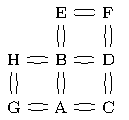
\includegraphics[height=\myMinHeight]{../../img/epsfromtikz/bodypin_graph}
        \caption{}\label{fig:bodypindrp:b}
    \end{subfigure}
    %
    \hfill
    \begin{subfigure}{0.35\linewidth}\centering
        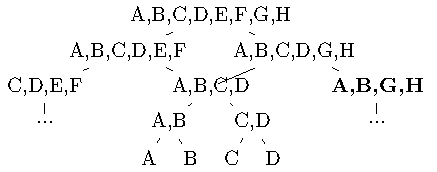
\includegraphics[height=\myMinHeight]{../../img/epsfromtikz/bodypin_drp}
        \caption{}\label{fig:bodypindrp:c}
    \end{subfigure}
    %
    \hfill
    \begin{subfigure}{0.2\linewidth}\centering
        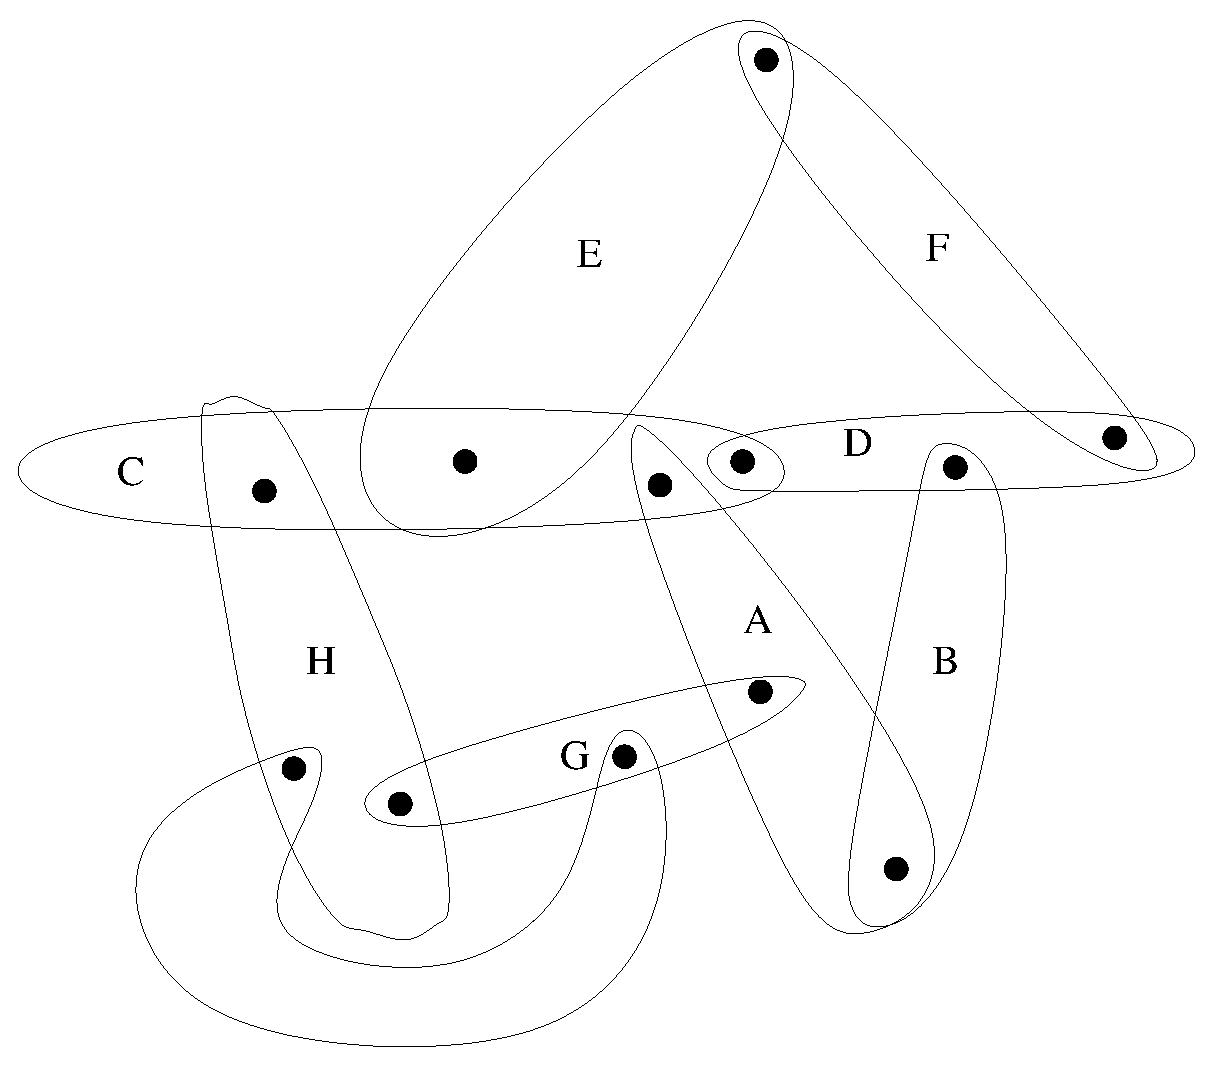
\includegraphics[height=\myMinHeight]{../../img/bodypin2}
        \caption{}\label{fig:bodypindrp:d}
    \end{subfigure}
    %
    \caption{(\ref{fig:bodypindrp:a}) A 1-dof body-pin graph. (\ref{fig:bodypindrp:b}) The corresponding body-bar graph, explained in Definition \ref{def:body-pin}. (\ref{fig:bodypindrp:c}) The 1-dof DR-plan for the graph. In this case, to obtain an isostatic system, we would need to add a body and 2 pins to one of the nodes in the second level. (\ref{fig:bodypindrp:d}) The result of adding one such body to the bold-faced node.}
    \label{fig:bodypindrp}
    %
\end{figure*}

The above discussion leads to the main theorem:
\begin{theorem*}
\label{thm:1dofcase}
    Given a 1-dof body-pin or triangle-multipin graph and corresponding 1-dof DR-plan, there is a quadratic algorithm for the 1-dof optimal completion problem of Section \ref{sec:recomb}.
\end{theorem*}

% \begin{proof}
%     Suppose we are given a body-pin graph and its corresponding body-bar graph $G$ and have obtained the 1-dof DR-plan $T$. Each node of $T$ will then be a vertex maximal proper 1-dof subgraph of $G$.

%     To make the graph isostatic, we need only add one body and pin it to 2 other bodies. Doing so will cause $G$ to become $(3,3)$-tight. We choose the 2 bodies to pin to by choosing a node $b$ in $T$ and looking at its children. From Observation \ref{rem:1dofcanon}, we know that the children can only be joined by a single pin or a subgraph. We pin the new body to bodies in two separate children. Doing so will ensure that all children of $b$ will have 1-dof and all ancestors of $b$ (including $b$) will now be isostatic.

%     % Then, we can form a valid isostatic DR-plan $T_b$ from $T$. In $T_b$, $fanin(b)$is the number of leaves in the subtree rooted at $b$ because no child of $b$ in $T$ is isostatic. Similarly, for any other node $w$ that is an ancestor of $b$, $fanin(w)$ is the the number leaf nodes in the tree rooted at $w$, excluding the subtree constaining $b$, plus 1 (for the node leading to $b$).  Then, for any node $b$ that we choose, $T_b$ is a valid DR-plan. The size of $T_b$ will just be the maximum fanin of all nodes in $T_b$. Thus, if we want to minimize the size of our DR-plan, we simply need to take the $b$ that has the $T_b$ of smallest size.

%     Such a pinning covers all possible ways of adding a new body. Assume we add a new body $b$ to our graph and pin it to $b_i$ and $b_j$ to make it isostatic. Then, there will be some lowest 1-dof node $v$ in $T$ such that $b_i$ and $b_j$ appear in $v$. Thus, pinning $v$ in the manner described yields an equivalent isostatic DR-plan to pinning $b$ to $b_i$ and $b_j$.

%     For each node $b$, we assign a size of the $T_b$ denoted $|T_b|$. $|T_b| = \displaystyle\max_{v \in T_b} fanin(v)$. We are looking for $b$ that minimizes $|T_b|$. Denote the sub-tree of $T$ rooted at $v$ by $T^v$ and the number of leaves in a tree $T$ by $nl(T)$. Note that $fanin(b)= nl(T^b)$ because no descendant of $b$ is isostatic. Similarly, for any ancestor $w$ of $b$, $fanin(w) = nl(T^w)-nl(T^{b'})+1$, where $b'$ is the child leading to $b$. All other nodes are not isostatic and so have no fanin.

%     % Then, we can form a valid isostatic DR-plan $T_b$ from $T$. In $T_b$, $b$'s children are now all of the leaf nodes of the subtree rooted at $b$ because no child of $b$ in $T$ is isostatic. Similarly, for any other node $w$ that is an ancestor of $b$, $w$'s children will be the node that leads to $b$, denoted $b'$, along with all of the other leaf nodes in the tree rooted at $w$, excluding $b'$. Then, for any node $b$ that we choose, $T_b$ is a valid DR-plan. The size of $T_b$ will just be the maximum fanin of all nodes in $T_b$. Thus, if we want to minimize the size of our DR-plan, we simply need to take the $b$ that has the $T_b$ of smallest size.

%     The node we need to pin will always be the deepest nontrivial node of some path in $T$. Suppose we chose to pin a node $b$ that has a nontrivial child $v$. Then, $fanin_b(b) = nl(T^b) = nl(T^v) + n$, where $n$ is essentially the number of leaves between $b$ and $v$. If we had instead chosen to pin $v$, then $fanin_v(b) = nl(T^b) - nl(T^{b'}) + 1 \leq fanin_b(v)$. And for each ancestor $w$ of $b$, $fanin(w)$ is unchanged, meaning $|T_v| \leq |T_b|$. Thus we only have to check the deepest non-trivial nodes.

%     Running this algorithm in a brute force fashion is quadratic in the number of bodies of our given body-pin system.

%     For the multi-triangle pin graphs, we can do the same thing except we need to add a single triangle to one of the nodes to cause it to become isostatic.
%     % Don't leave a blank line between last paragraph and end!
%     % For the 2-dof case, we can do something very similar, except instead of pinning a single body 2 times to a node, we can pin another body 2 times to a node. These can be the same node, and if it is the same node, we can find a wellconstrained DR-plan in quadratic time, we would just be doing the same thing as the 1-dof case.
% \end{proof}

\begin{observation*}
\label{obs:2dof_case}
    For the 2-dof case, provided an analogous statement to Observation \ref{rem:1dofcanon} holds, then Theorem \ref{thm:1dofcase} holds for the 2-dof  systems.
\end{observation*}

% \begin{proof} (of Observation \ref{obs:2dof_case})
%     The only difference from the 1-dof case is that now we need to remove 2-dof from our graph. We build a 2-dof DR-plan $T$. Like above, we need to add a body and 2 pins to 2 nodes now to get to isostatic.

%     Suppose we pin 2 distinct nodes $v_i$ and $v_j$. Then, there will be some common ancestor $a$ of $v_i$ and $v_j$. Then, in $T_{v_i,v_j}$, $fanin_{v_i,v_j}(a) = nl(T^a)$. However, if we chose to pin one of $v_i$ and $v_j$ twice, then $fanin_v(a) = nl(T^a) - nl(T^{a'}) +1$ . Thus $fanin_v(a)' \leq fanin_{v_i,v_j}(a)$. All ancestors of $a$ are unchanged. So $|T_v| \leq |T_{v_i,v_j}|$.

%     So, we will always end up pinning a single node twice. Hence, we can run the same algorithm as the 1-dof case and just pin twice instead of once.
% \end{proof}

\begin{remark}
\label{obs:algebraic_completion}
    While the proof for Theorem \ref{thm:1dofcase} gives us a DR-plan for the isostatic completion with minimum fan-in (a reasonable measure of algebraic complexity), a more nuanced measure that treats solutions of 1-dof and 2-dof systems as 1 or 2 parameter families would no longer be optimized by the algorithm given in that proof. In particular, the complexity of the standard algorithm in the $k$-dof case would be exponential in $k$ (even if the case were matroidal and an optimal DR-plan is known).
\end{remark}

% \begin{proof}
%     An isostatic graph has 3 parameters that define it (in terms of coming up with a realizaiton). These are the Euclidean motions. A 1-dof graph can be seen as essentially having 4 parameters: the 3 Euclidean motions and whatever degree of freedom it has. A 2-dof has 5 parameters, and so on. These paramters denote the algebraic complexity of giving a realization for the graphs.

%     Thus, say we have a $T$ as described in the proof for Theorem \ref{thm:1dofcase}. When we pin a node $b$, we will have the same structure as before. Suppose we are looking at an isostatic node $v$ after pinning $b$. Then, the children of $v$ (except one if $v \neq b$) will be 1-dof. The complexity for that node is then just that of solving each of its children. In general then, the number of parameters for that node will be $np(v) = 4nc_1(v)+3$, if $v \neq b$ and $np(b) = 4nc_1(b)$, where $nc_k(v)$ is the number of $k$-dof children of $v$.

%     Now if we want to minimize the algebraic complexity, we need to minimize the maximum $np(v)$ for any node $v$. In this case, we cannot always just choose the node furthest down the tree to pin because it could have many children. So we will have to try pinning all nodes to see which gives the lowest algebraic complexity. This is still quadratic for the 1-dof case.

%     For the 2-dof case, there are more cases to consider. If we pin the same node twice as above, we have $np(v) = 5nc_2(v)+3$ for any ancestor $v \neq b$ and $np(b) = 5nc_2(b)$. If we pin a node $v$ and one of its ancestors $v'$, then any nodes between $v'$ and $v$ will be 1-dof, any nodes above $v'$ will be isostatic, and nodes below $v$ will be 2-dof. Note that solving $v'$ will result in solving $v$. Then, we need to consider nodes above and includiing $v'$ in our complexity. $np(v') = 5nc_2(v') + 4$ and $np(a) = 3 + 5nc_2(a)$ for $a$ an ancestor of $v'$. The only remaining case will be if we pin two nodes that are not descendent/ancestor. the only change from the previous case will be that for the lowest common ancestor of the nodes $v'$, $np(v') = 2*4+5nc_2(v')$. For any ancestor $a$ of $v'$, we still have $np(a) = 3 + 5nc_2(a)$.

%     Like the 1-dof case, we again cannot just choose the nodes deepest in the tree to pin. However, we cannot also assume pinning one node twice will give us the best algebraic complexity. Hence, we will need to check each pair of node to pin. This makes our brute-force algorithm $O(b^3)$, where $b$ is the number of bodies.
% \end{proof}
